%   Filename    : chapter_4.tex 
\chapter{Preliminary Results/System Prototype}
\section{Data Gathering}
The data for dengue case prediction was gathered from a variety of reliable sources, enabling a comprehensive dataset spanning from January 2016 to September 2024. This dataset includes 452 rows of data, each containing weekly records of dengue cases along with corresponding meteorological variables, such as rainfall, temperature, and humidity.
\begin{enumerate}
	\item Dengue Case Data: The primary source of historical dengue cases came from the Humanitarian Data Exchange and the Western Visayas Center for Health Development (WVCHD). The dataset, accessed through Freedom of Information (FOI) requests, provided robust case numbers for the Western Visayas region. The systematic collection of these data points was essential for establishing a reliable baseline for model training and evaluation.
	\item Weather Data: Weekly weather data was obtained by web scraping from Weather Underground, allowing access to rainfall, temperature, and humidity levels that correlate with dengue prevalence.
\end{enumerate}

\begin{figure}[ht]
	\centering
	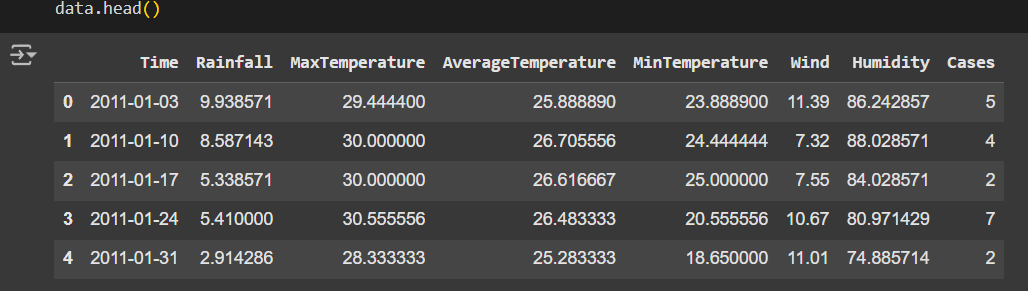
\includegraphics[width=0.75\textwidth]{data_snippet}
	\caption{Snippet of the Combined Dataset}
	\label{fig:data_snippet}
\end{figure}

\section{Preliminary Model Training}
The proposed Dengue Watch system utilized four distinct models to forecast weekly dengue cases: Long Short-Term Memory (LSTM) networks, Autoregressive Integrated Moving Average (ARIMA), Seasonal ARIMA (SARIMA), and Kalman Filter. Each model was trained on a dataset containing 452 weeks of historical dengue cases from 2016 to 2024, with meteorological variables such as temperature, humidity, and rainfall.

To optimize predictive performance, hyperparameter tuning was conducted individually for each model, refining parameters to achieve the most accurate and reliable forecasts. Following training, the models were rigorously evaluated against the dataset using a set of key performance metrics, including Mean Squared Error (MSE) and Root Mean Squared Error (RMSE).

The table below provides a summary and comparative analysis of each model’s results across these metrics, offering insights into the strengths and limitations of each forecasting technique for dengue case prediction in Iloilo City. 

\begin{table}[h!]
	\centering
	\begin{tabular}{|l|c|c|}
		\hline
		\textbf{Model} & \textbf{MSE} & \textbf{RMSE} \\ \hline
		\textbf{LSTM} & \textbf{342.59} & \textbf{18.51} \\ \hline
		\begin{tabular}[c]{@{}l@{}}\textbf{Seasonal ARIMA} \\ \textbf{(2, 0, 2) (0, 1,1)}\end{tabular} & \textbf{1198} & \textbf{34.62} \\ \hline
		\textbf{ARIMA (2, 0, 3)} & \textbf{1983.16} & \textbf{44.53} \\ \hline
		\textbf{Kalman Filter} & \textbf{2755.77} & \textbf{52.49} \\ \hline
	\end{tabular}
	\caption{Comparison of Models}
	\label{tab:comparison_of_models}
\end{table}

\subsection{LSTM Model}
The LSTM model architecture consisted of an input layer, a single LSTM layer with 64 units and ReLU activation, followed by a dense layer with a single output neuron to predict the dengue case count. Key hyperparameters included:
\begin{itemize}
	\item Window Size: 10 weeks, representing the time steps used in the sequence data for each prediction.
	\item Epochs: 50 epochs were used for training, balancing sufficient training time with computational efficiency.
	\item Batch Size: 1, allowing the model to process one sequence at a time, which is beneficial for small datasets but increases training time.
	\item Optimizer: The Adam optimizer was chosen for its adaptive learning capabilities and stability in training. A custom learning rate of 0.0001 was set to ensure gradual convergence and minimize risk of overfitting.
\end{itemize}

Data Division for Training and Testing
The dataset was split into training and test sets to evaluate the model’s performance and generalizability:
\begin{itemize}
	\item Training Set: 85\% of the data (385 sequences) was used for model training, enabling the LSTM to learn underlying patterns in historical dengue case trends and their relationship with weather variables.
	\item Test Set: The remaining 15\% of the data (67 sequences) was reserved for testing
\end{itemize}

Upon testing, the LSTM model produced an MSE of 342.59 and an RMSE of 18.51, showing its capability to generalize to unseen data. The close alignment of actual and predicted values in the test set plot supports this observation, suggesting that the model successfully captured critical temporal trends that correlate with dengue outbreaks.

\begin{figure}[H]
	\centering
	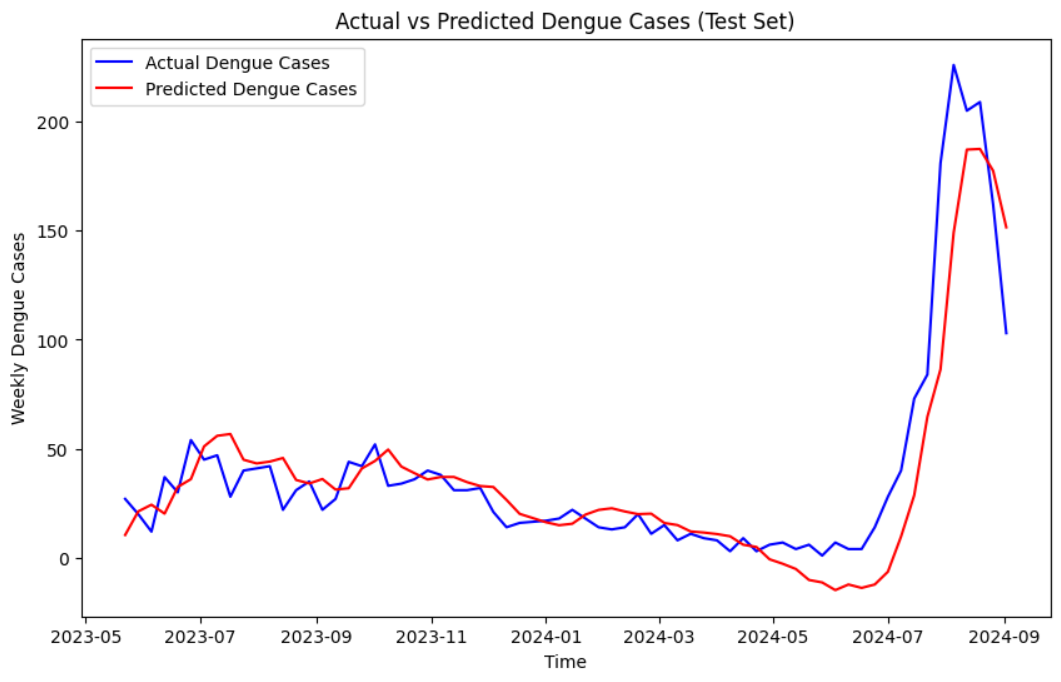
\includegraphics[width=1\textwidth]{line_graph_LSTM}
	\caption{LSTM Prediction Results for Test Set}
	\label{fig:LSTM_result}
\end{figure}

\section*{Training and Testing Data Division for ARIMA and Seasonal Arima}
Both models utilized an \textbf{80\%-20\% split} to evaluate generalizability:
\begin{itemize}
	\item \textbf{Training Set}: 80\% of the data was used for training, allowing the models to learn underlying patterns in the dataset.
	\item \textbf{Test Set}: 20\% of the data was reserved for testing, providing an unbiased assessment of the models' performance on unseen data.
\end{itemize}
\subsection{ARIMA Model}

\begin{figure}[H]
	\centering
	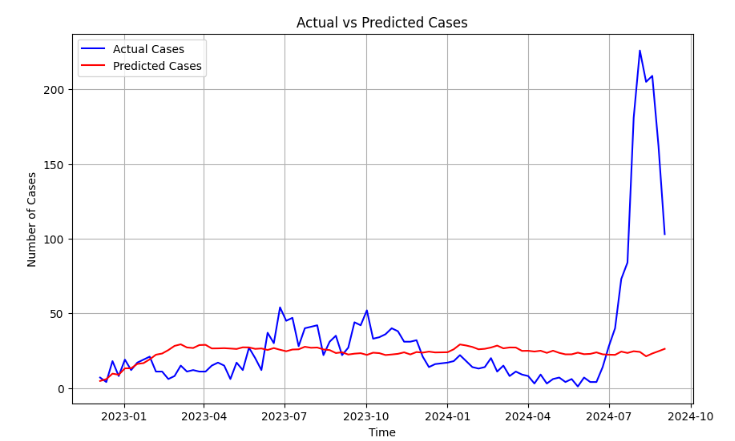
\includegraphics[width=1\textwidth]{line_graph_Arima}
	\caption{ARIMA Prediction Results for Test Set}
	\label{fig:Arima_result}
\end{figure}

The ARIMA model was developed to capture non-seasonal trends in the data. To determine the best model configuration, grid search was used to explore various combinations of ARIMA parameters, ultimately selecting \textbf{ARIMA(2, 0, 3)}. The model was iteratively refined over \textbf{400 iterations} to ensure convergence to an optimal solution. Key details are as follows:

\begin{enumerate}
	\item \textbf{Data Preprocessing:}  
	Prepare the dataset by handling any missing values and scaling the data if necessary to improve model convergence and stability.
	
	\item \textbf{Hyperparameter Tuning:}  
	Use a grid search on potential ARIMA parameters $(p, d, q)$ to identify the configuration that minimizes error. The optimal parameters were found to be \textbf{(2, 0, 3)}.
	
	\item \textbf{Model Training:}
	\begin{itemize}
		\item Set the number of iterations to 400 to ensure thorough training and convergence.
		\item Train the ARIMA model on 80\% of the data and reserve 20\% for testing.
	\end{itemize}
	
	\item \textbf{Evaluation:}  
	After training, the ARIMA model was evaluated on the test data, yielding the following performance metrics:
	\begin{itemize}
		\item \textbf{MSE (Mean Squared Error)}: 1983.16
		\item \textbf{RMSE (Root Mean Squared Error)}: 44.53
	\end{itemize}
\end{enumerate}


\section*{Seasonal ARIMA (SARIMA) Model}

\begin{figure}[H]
	\centering
	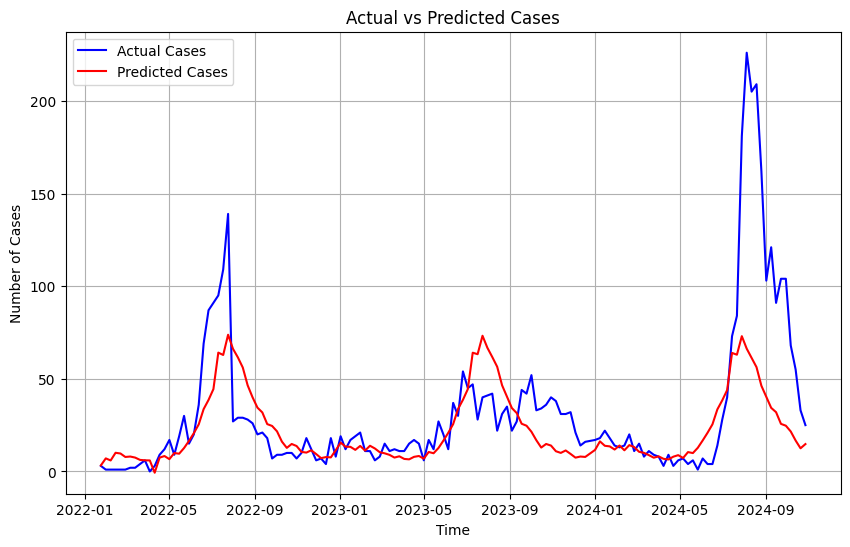
\includegraphics[width=1\textwidth]{line_graph_Sarima}
	\caption{Seasonal ARIMA Prediction Results for Test Set}
	\label{fig:Sarima_result}
\end{figure}

This model incorporates seasonal parameters, which were tuned using grid search to find the best configuration: \textbf{SARIMA(2, 0, 2)(0, 1, 1)[52]}. As with ARIMA, \textbf{400 iterations} were applied to ensure a robust fit.

\subsection*{Steps to Create the SARIMA Model:}
\begin{enumerate}
	\item \textbf{Data Preprocessing:}  
	Ensure data readiness by filling any missing values and scaling as needed.
	
	\item \textbf{Seasonality Analysis:}  
	Examine the dataset for seasonal patterns. A periodicity of \textbf{52 weeks} was identified, making SARIMA a suitable choice for capturing yearly seasonality.
	
	\item \textbf{Hyperparameter Tuning:}  
	Conduct grid search to identify the best set of parameters $(p, d, q)(P, D, Q)[S]$, where:
	\begin{itemize}
		\item \textbf{(p, d, q)} are the non-seasonal parameters,
		\item \textbf{(P, D, Q)} are the seasonal parameters, and
		\item \textbf{S} is the season length.
	\end{itemize}
	The optimal configuration found was \textbf{(2, 0, 2)(0, 1, 1)[52]}.
	
	\item \textbf{Model Training:}
	\begin{itemize}
		\item Set the iteration count to 400 for enhanced model robustness.
		\item Train the model on the 80\% training dataset and reserve the remaining 20\% for testing.
	\end{itemize}
	
	\item \textbf{Evaluation:}  
	The SARIMA model yielded the following error metrics:
	\begin{itemize}
		\item \textbf{MSE}: 1198
		\item \textbf{RMSE}: 34.62
	\end{itemize}
	The SARIMA model outperformed the ARIMA model in terms of lower MSE and RMSE values, indicating its effectiveness in capturing the seasonal patterns in the data.
\end{enumerate}

\subsection{Kalman Filter Model}

\begin{figure}[H]
	\centering
	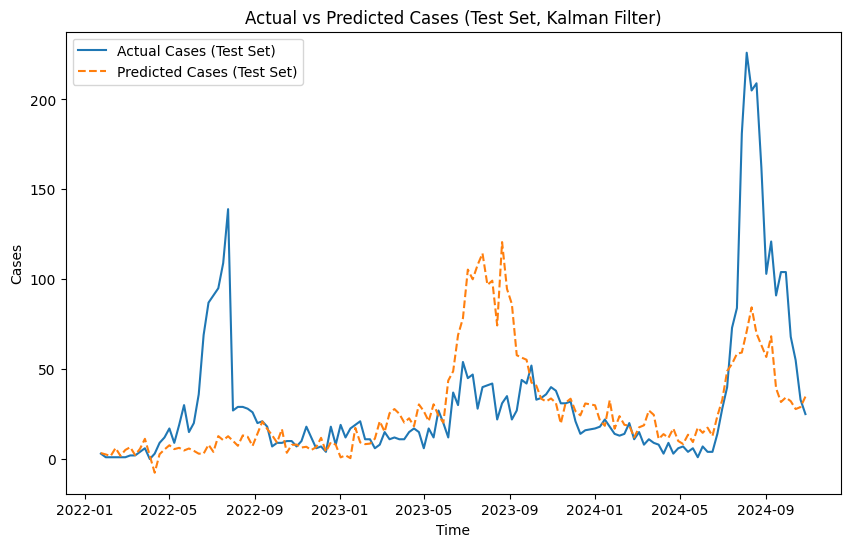
\includegraphics[width=1\textwidth]{line_graph_Kalman}
	\caption{Kalman Filter Prediction Results for Test Set}
	\label{fig:Kalman_result}
\end{figure}

\section*{Kalman Filter Methodology with Matrix Calculations}

\textbf{Measurement Acquisition}: Obtain the measurement \( z_k \) of the system's state with associated confidence. This measurement matrix provides a noisy observation of the true state.

The dataset was split into training and test sets to evaluate the Kalman Filter's performance and generalizability:
\begin{itemize}
	\item \textbf{Training Set}: 80\% of the data was used for training, enabling the Kalman Filter model to capture key patterns.
	\item \textbf{Test Set}: The remaining 20\% of the data was reserved for testing.
\end{itemize}

\textbf{Prediction Step}:
\begin{itemize}
	\item Predict the next state:
	\[
	\hat{x}_{k|k-1} = A \hat{x}_{k-1|k-1} + B u_k
	\]
	where \( A \) is the state transition matrix and \( B \) is the control matrix.
	
	\item Update the state covariance:
	\[
	P_{k|k-1} = A P_{k-1|k-1} A^T + Q
	\]
	where \( Q \) is the process noise covariance matrix.
\end{itemize}

\textbf{Compute Residual}: Calculate the residual
\[
y_k = z_k - H \hat{x}_{k|k-1}
\]
where \( H \) is the observation matrix. This residual represents the new information from the measurement.

\textbf{Scaling Factor (Kalman Gain)}:
\begin{itemize}
	\item Compute the Kalman Gain:
	\[
	K_k = P_{k|k-1} H^T (H P_{k|k-1} H^T + R)^{-1}
	\]
	where \( R \) is the measurement noise covariance matrix.
	
	\item The Kalman Gain determines the weight of the measurement relative to the prediction.
\end{itemize}

\textbf{State Update}:
\begin{itemize}
	\item Update the state estimate:
	\[
	\hat{x}_{k|k} = \hat{x}_{k|k-1} + K_k y_k
	\]
	blending the prediction and measurement.
\end{itemize}

\textbf{Uncertainty Update}:
\begin{itemize}
	\item Update the state covariance:
	\[
	P_{k|k} = (I - K_k H) P_{k|k-1}
	\]
	where \( I \) is the identity matrix.
\end{itemize}

\textbf{Model Evaluation}:
Upon testing, the Kalman Filter produced a Mean Squared Error (MSE) of 2755.77 and a Root Mean Squared Error (RMSE) of 52.49.

\clearpage
\section{Guest Interface}
The Guest Interface is intended for all visitors of the web application. It shows the related statistics for dengue cases in a particular area and time. As the system is still in its testing phase, the data converted into charts shown in Figure \ref{fig:guest_dashboard} are generated from Python's Faker library. 
\begin{figure}[H]
	\centering
	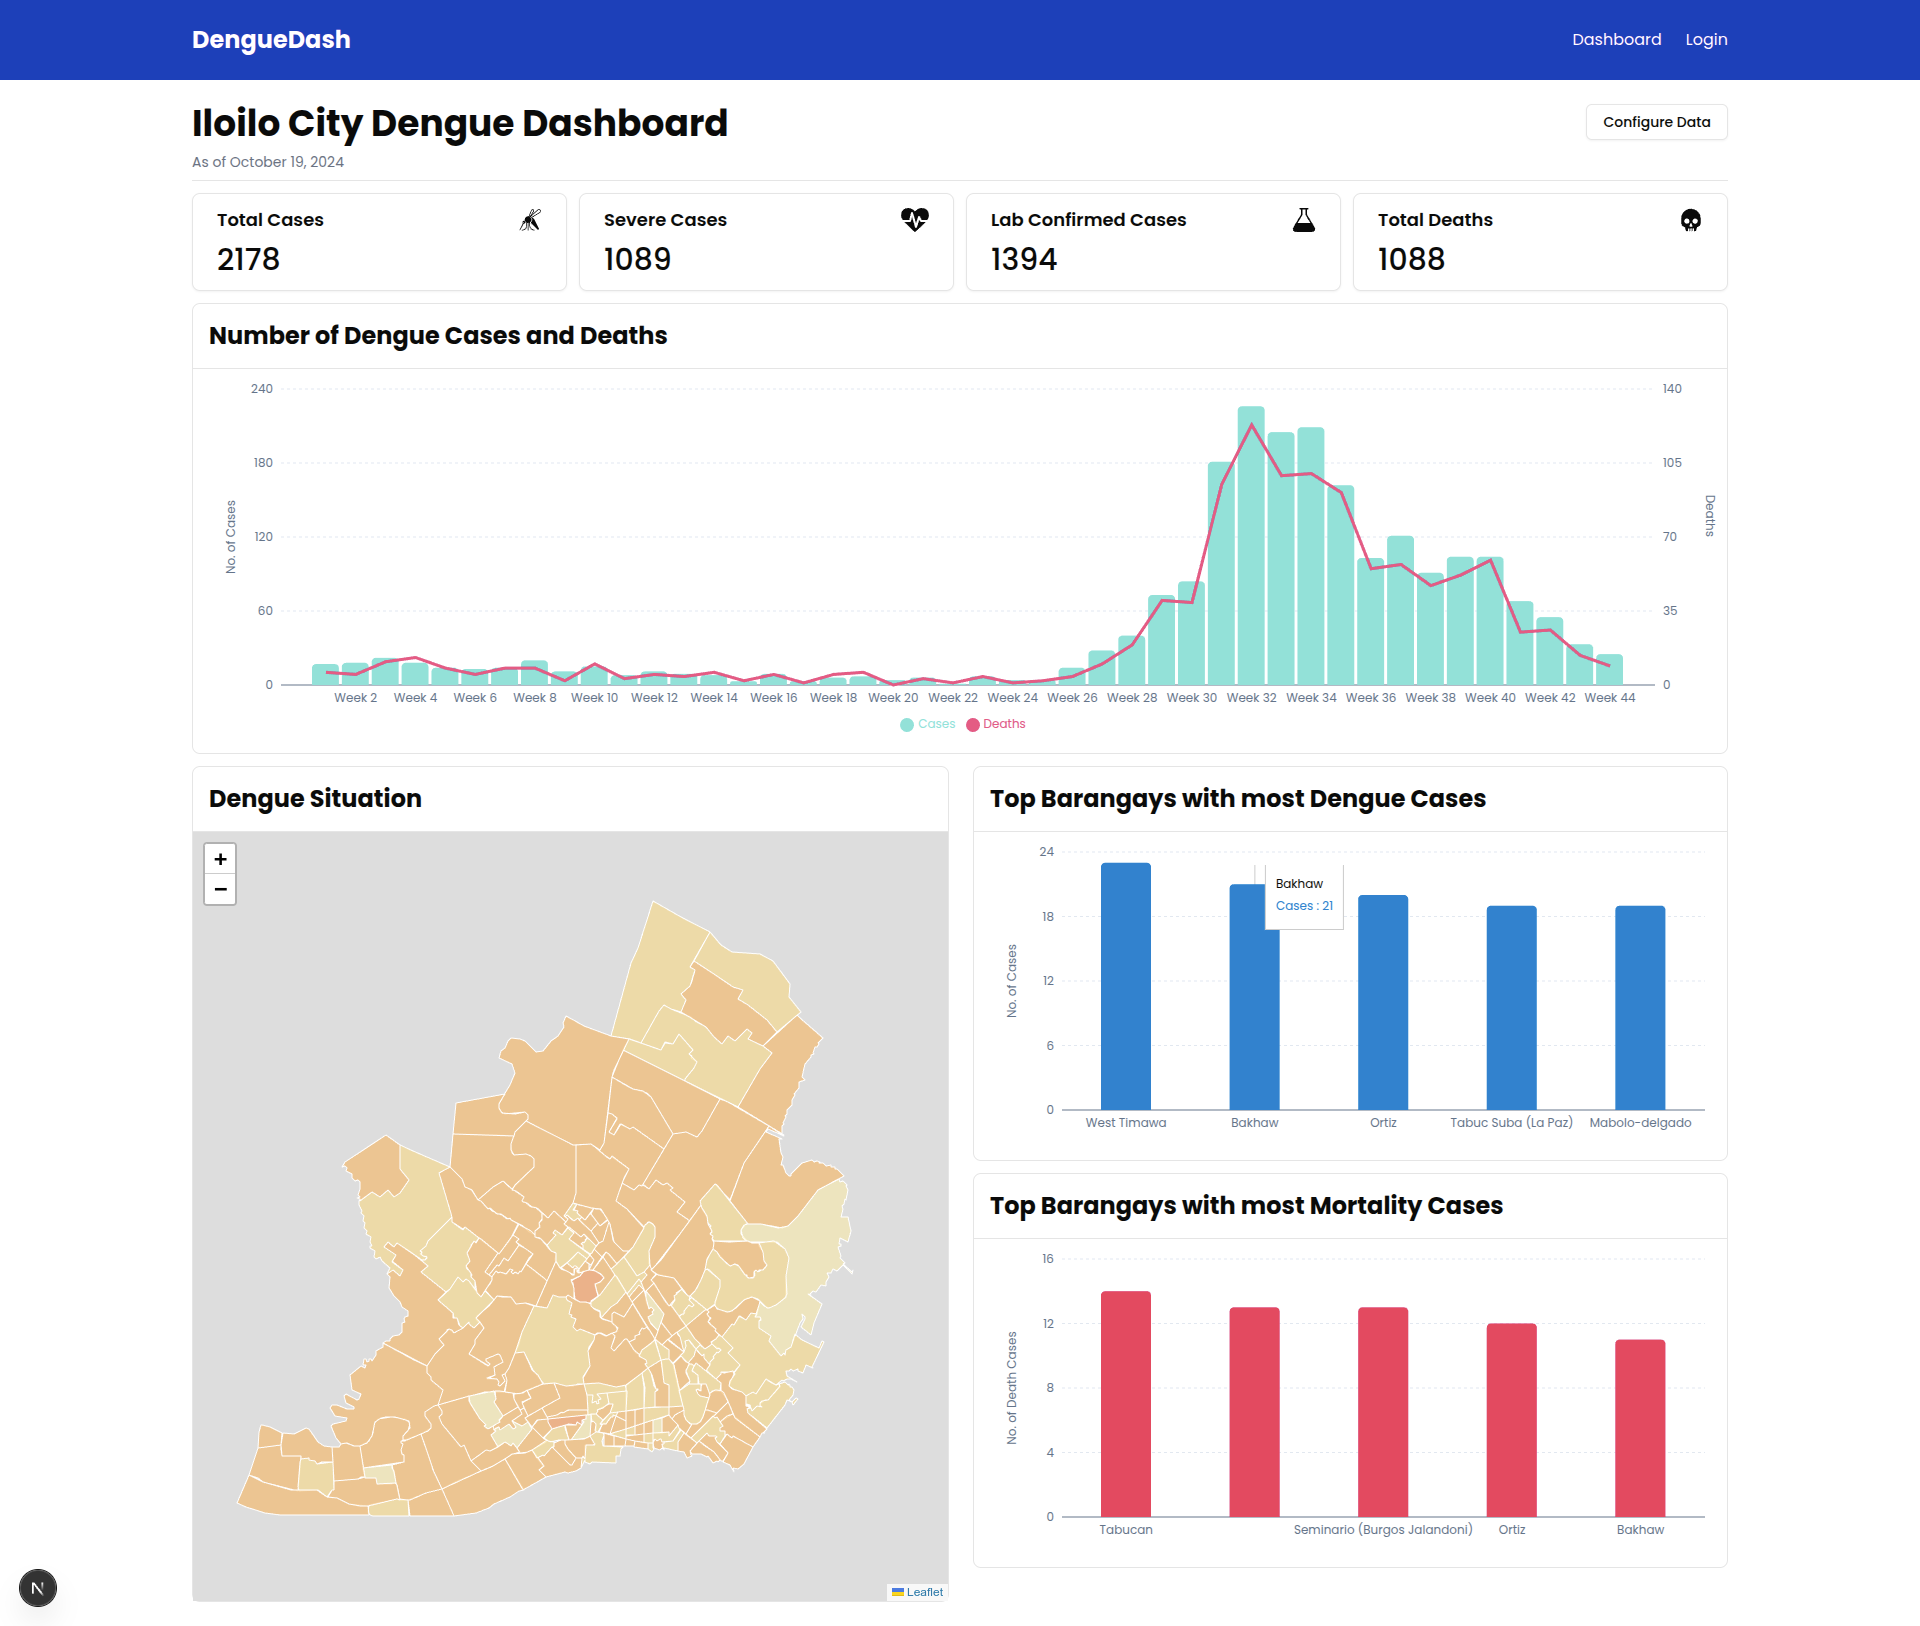
\includegraphics[width=1\textwidth]{guest_dashboard}
	\caption{Dashboard for Guests}
	\label{fig:guest_dashboard}
\end{figure}
\section{Personnel Interface}
\subsection{User Authentication, and Login}
To protect the data's integrity in production, it has been decided that the registration process will not be visible. Instead, an admin must register a user using a different interface. As of the moment, registering a user is done using API via Postman. In the login process, the system implements HTTP-only cookies that save the JSON Web Tokens (JWT) to protect against XSS attacks. After proper credentials have been provided, it will redirect to the user's home page.
\begin{figure}[H]
	\centering
	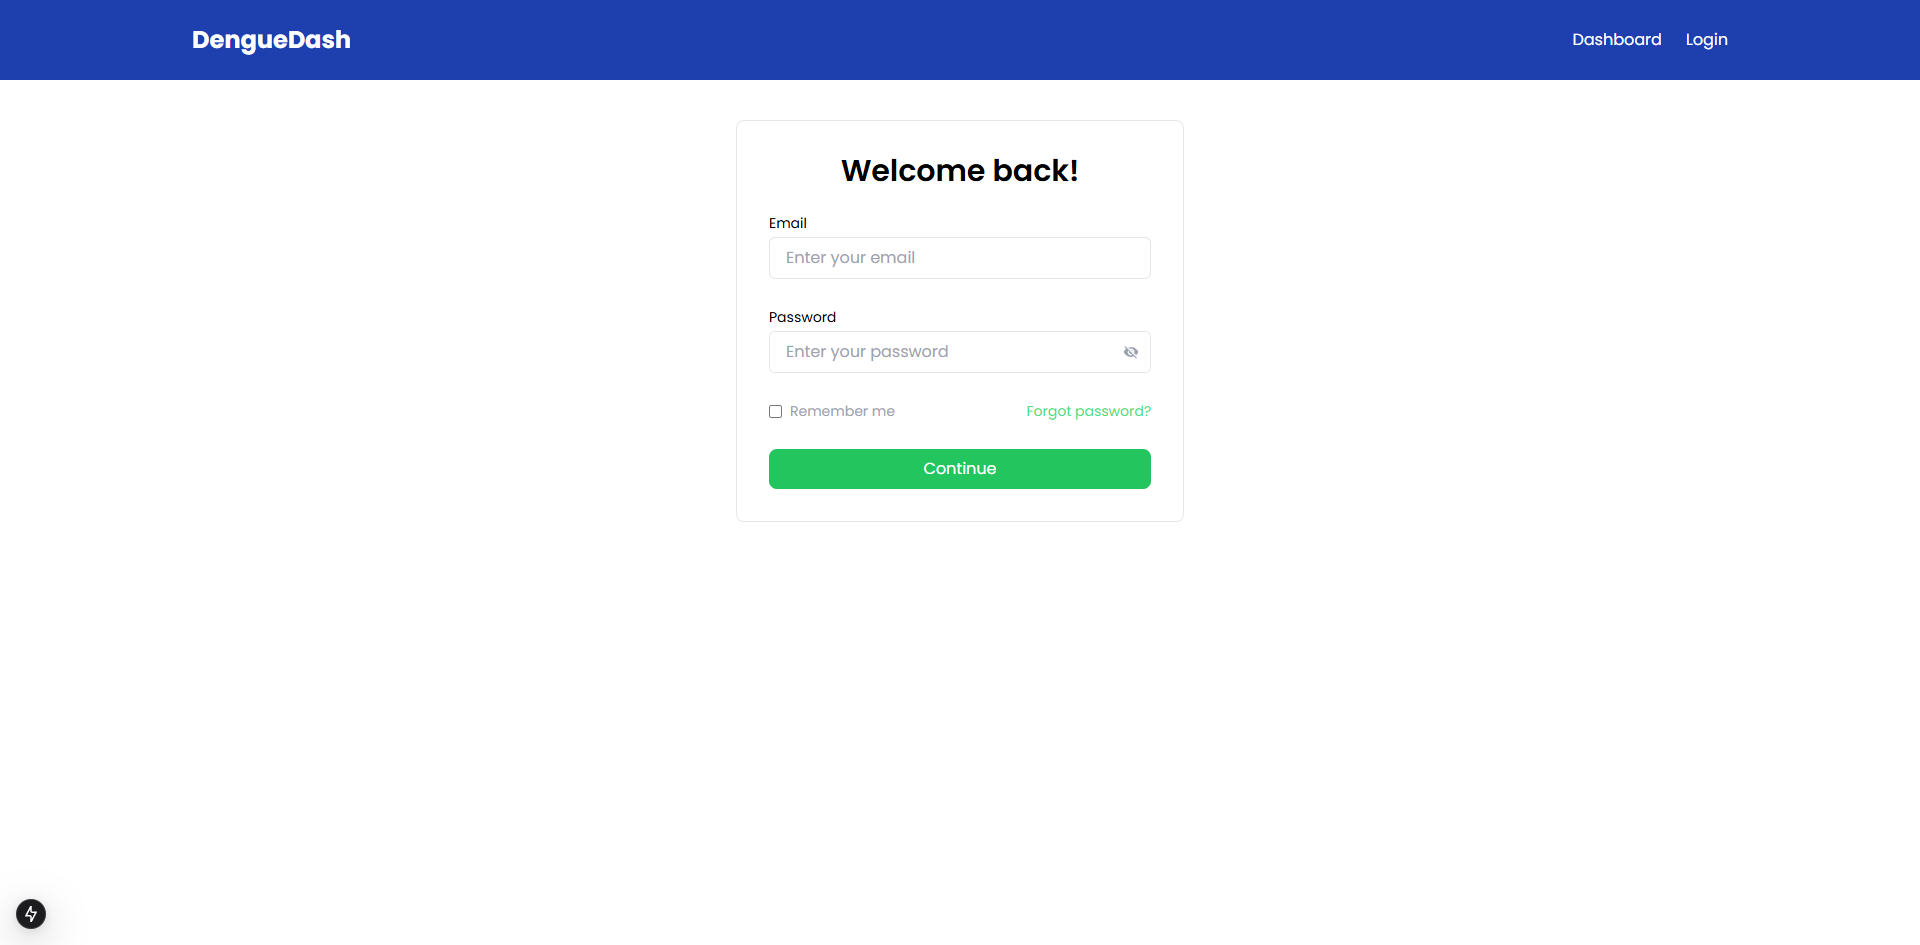
\includegraphics[width=1\textwidth]{login}
	\caption{Login Page for Users}
	\label{fig:login_page}
\end{figure}
\begin{figure}[H]
	\centering
	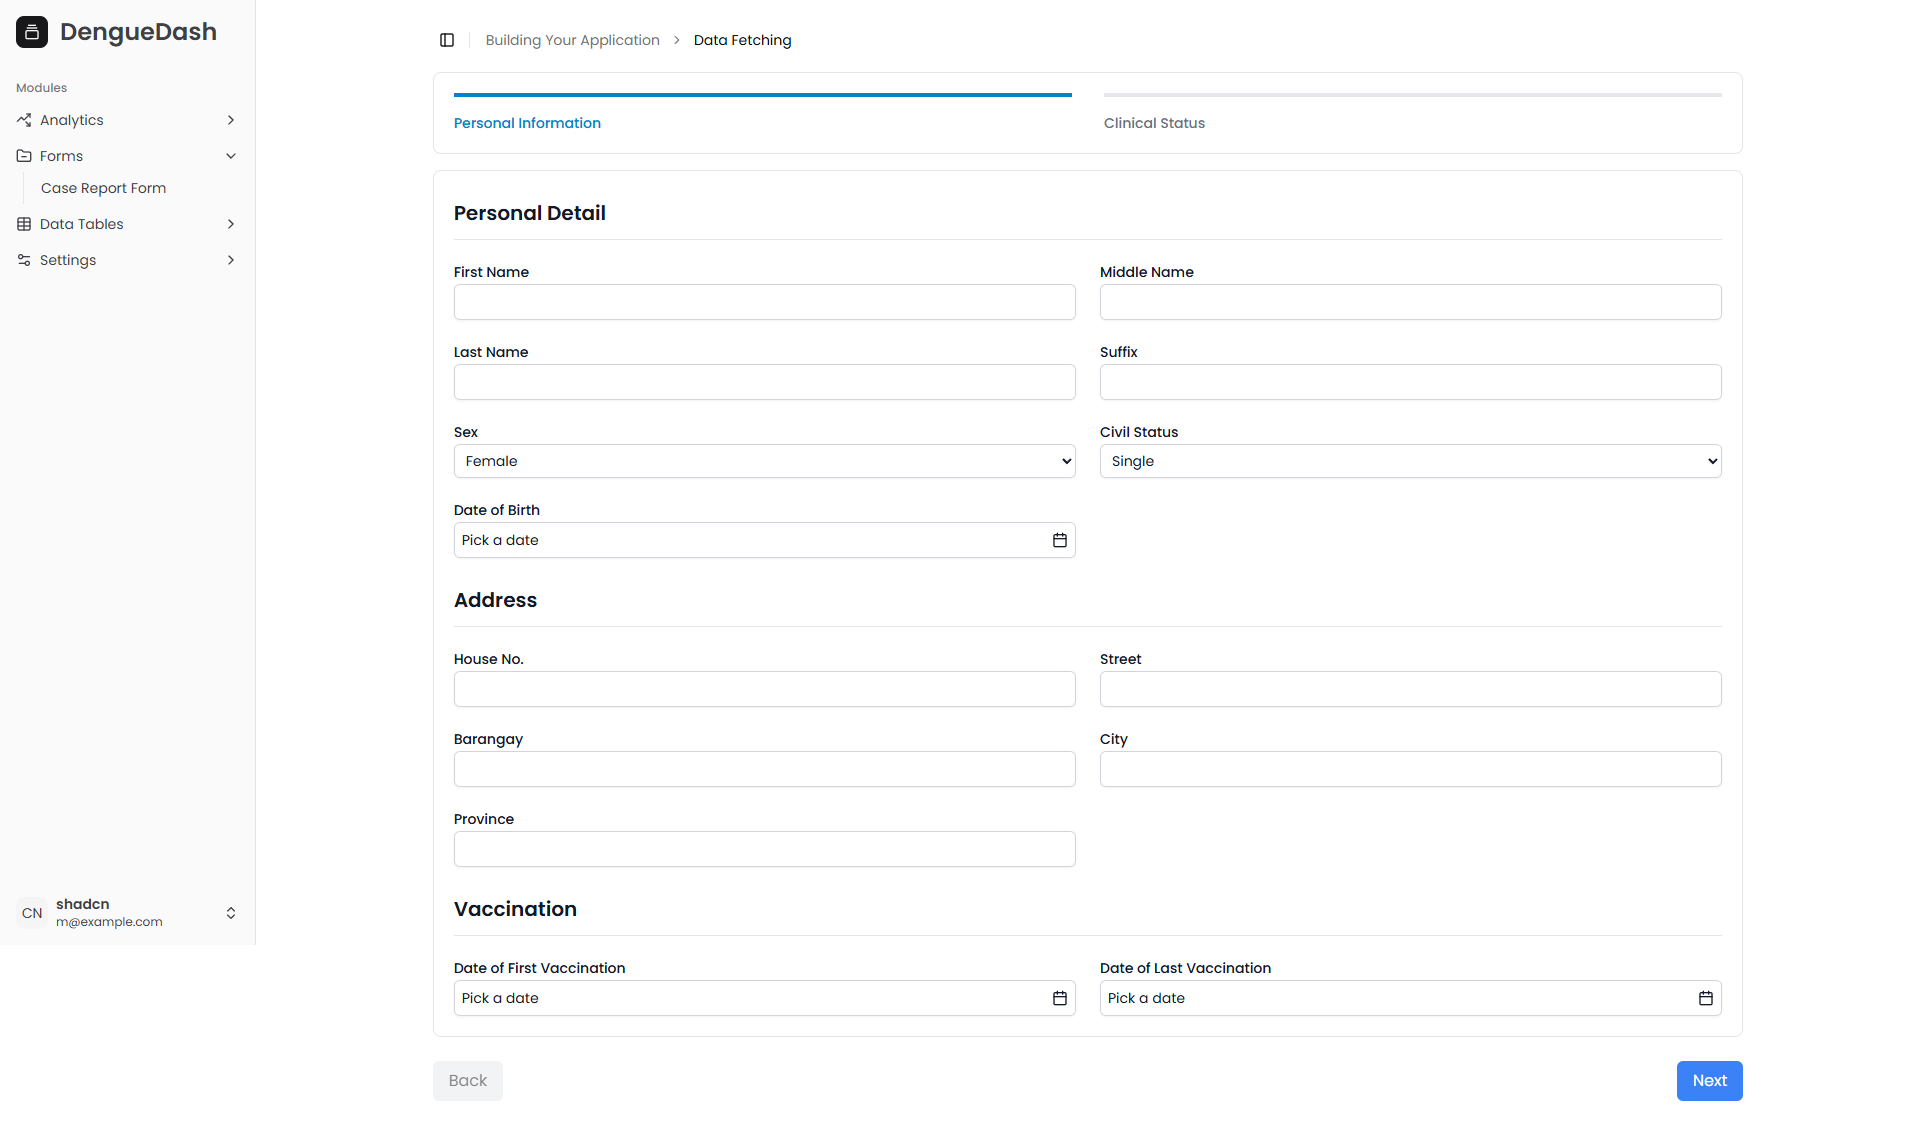
\includegraphics[width=1\textwidth]{case_report_form_1}
	\caption{First Part of Case Report Form}
	\label{fig:case_report_form_1}
\end{figure}
\begin{figure}[H]
	\centering
	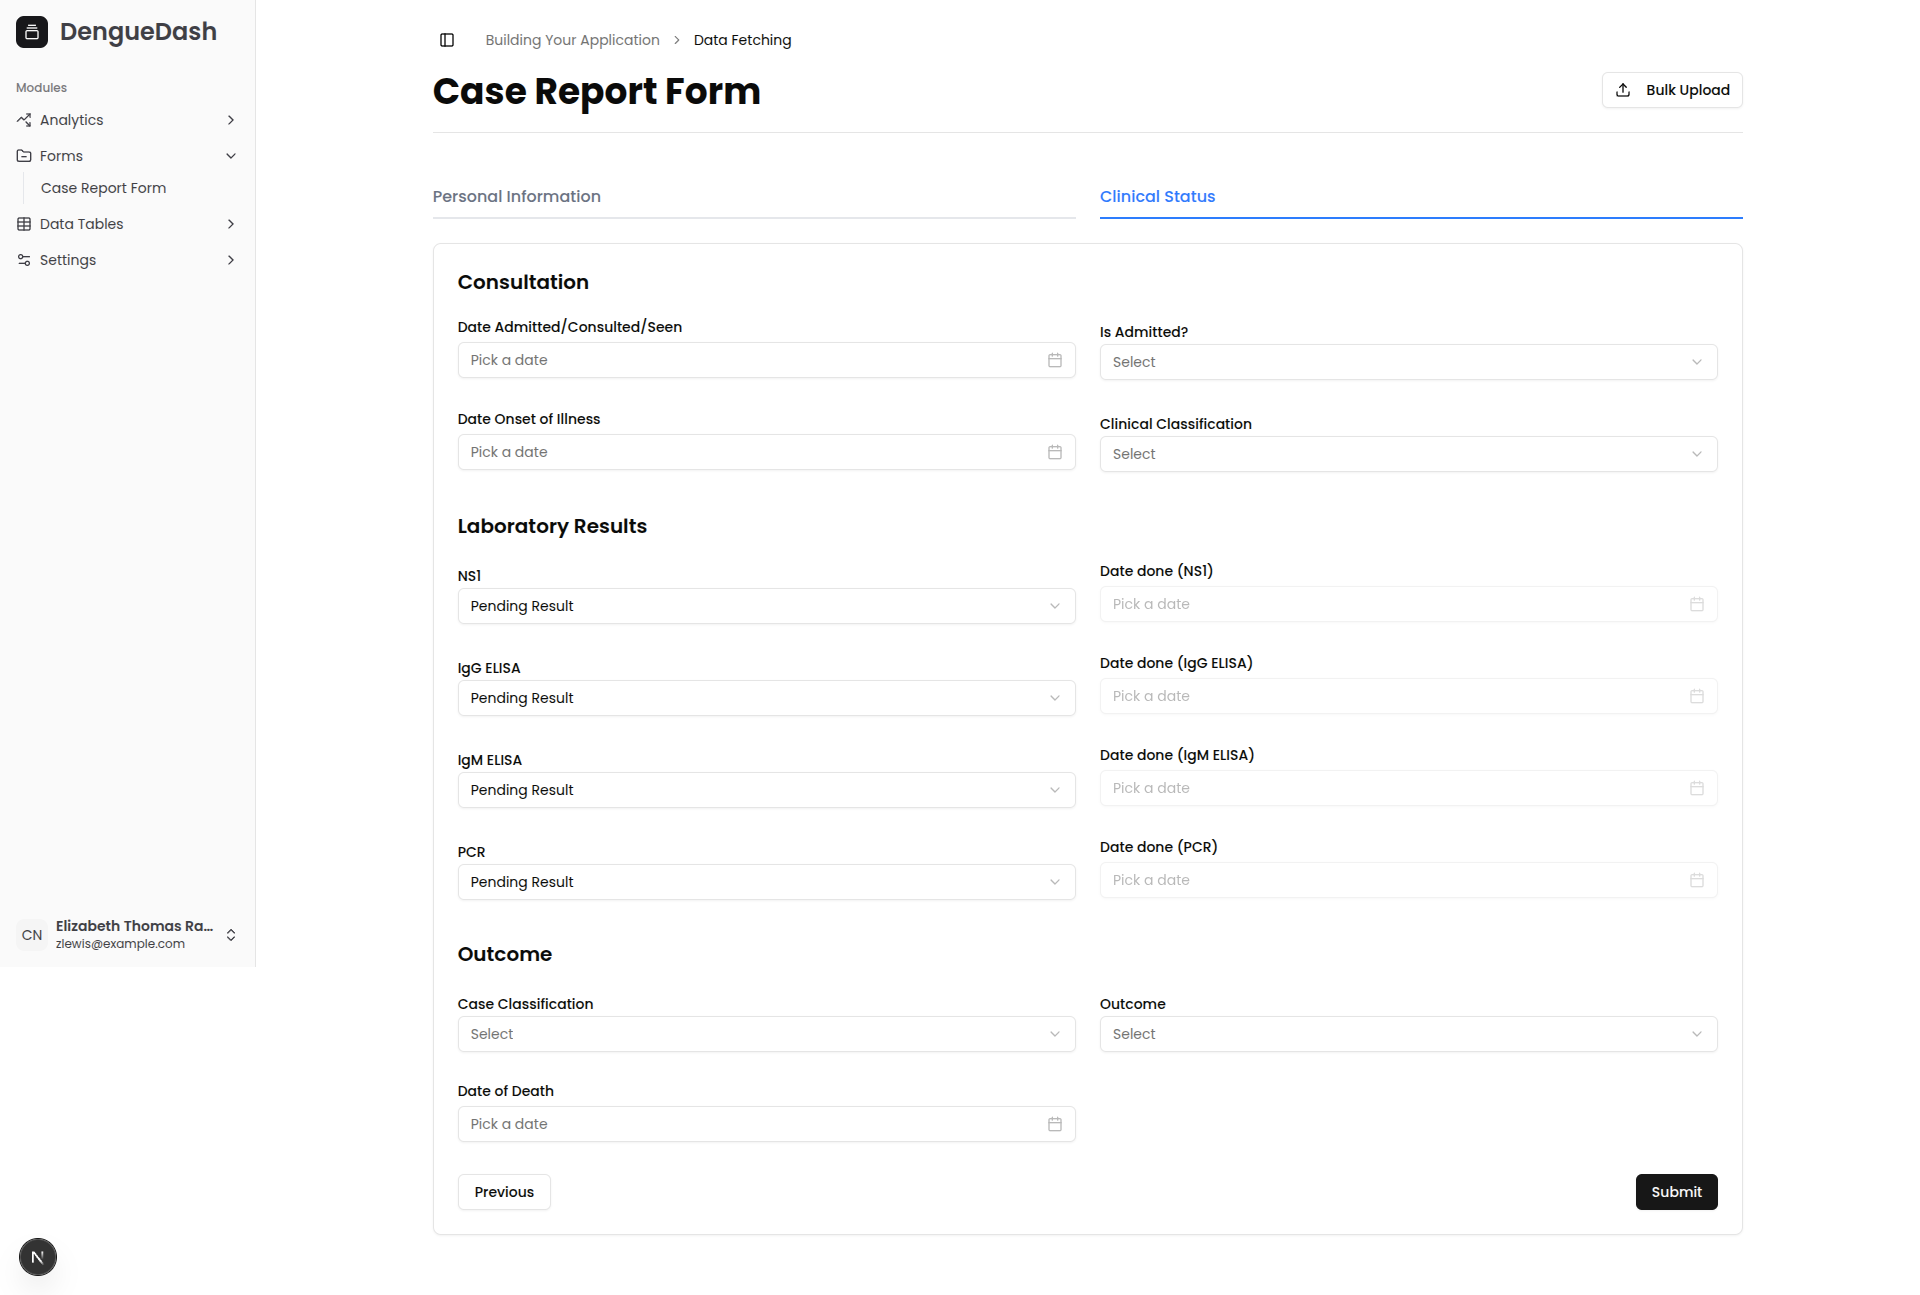
\includegraphics[width=1\textwidth]{case_report_form_2}
	\caption{Second Part of Case Report Form}
	\label{fig:case_report_form_2}
\end{figure}
\begin{figure}[H]
	\centering
	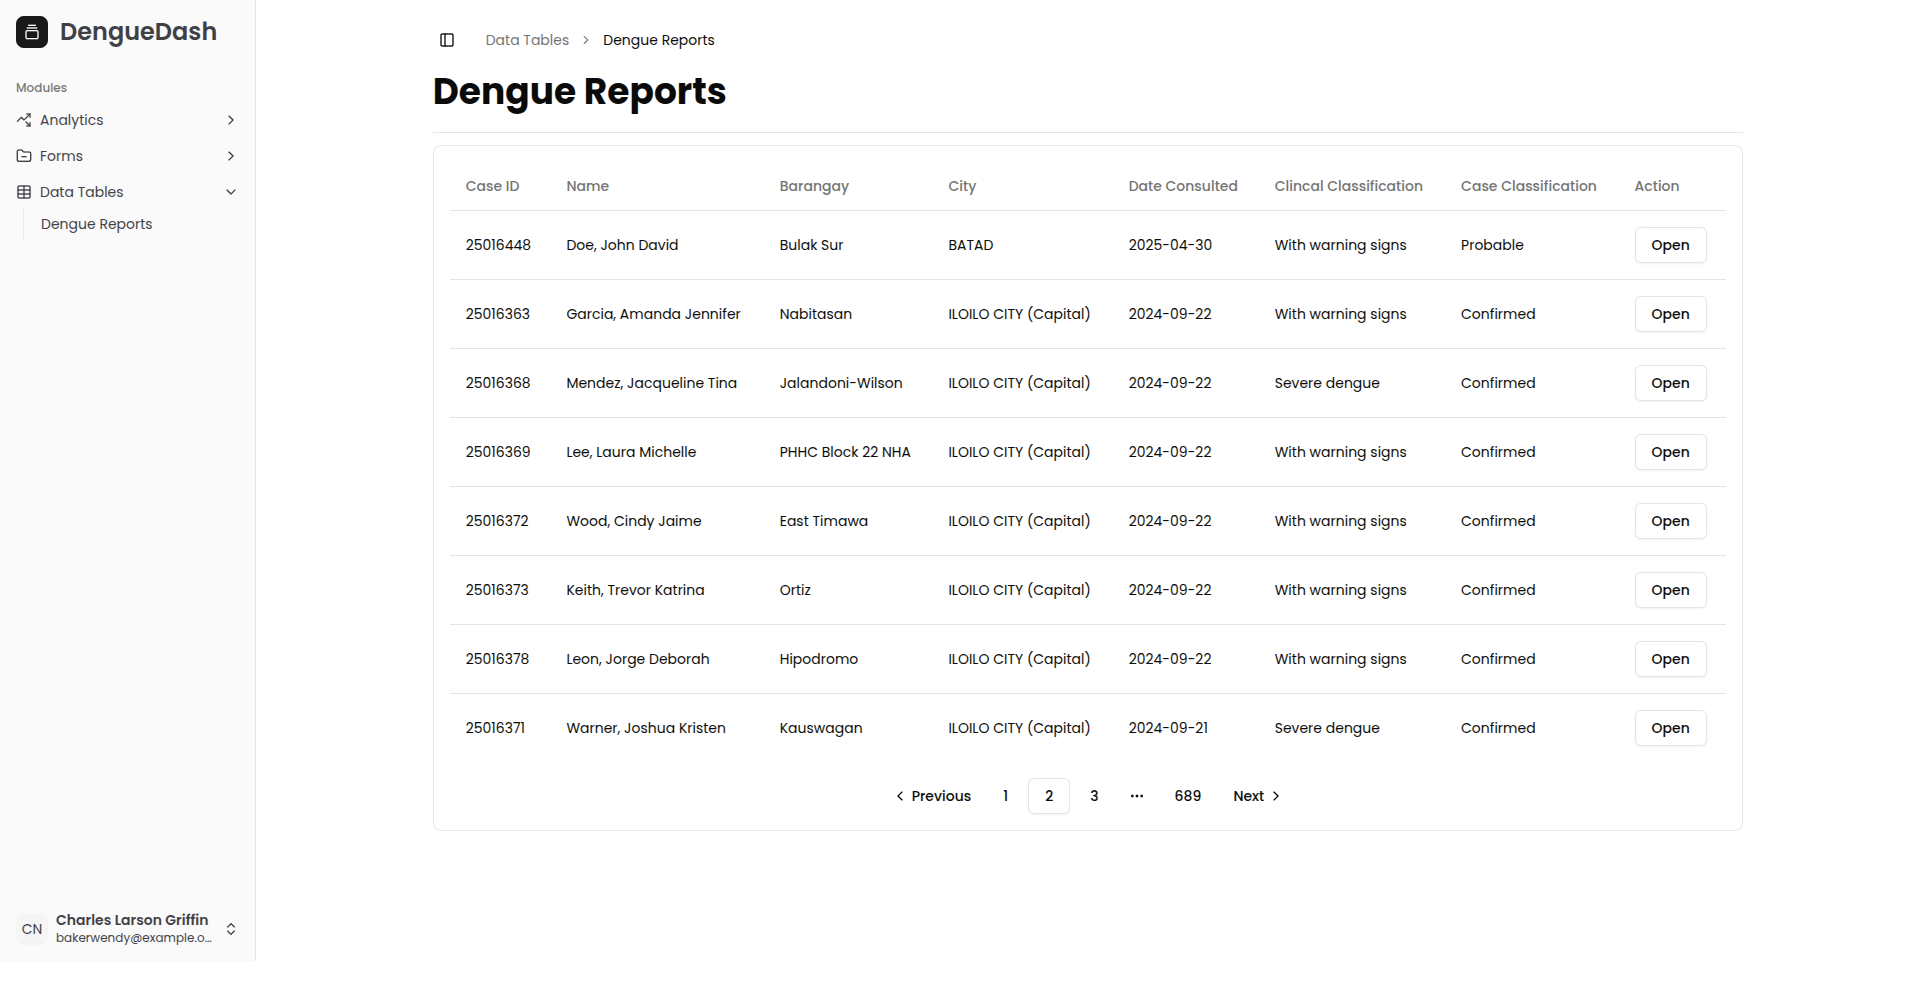
\includegraphics[width=1\textwidth]{dengue_reports}
	\caption{Dengue Reports}
	\label{fig:dengue_reports}
\end{figure}
\begin{figure}[H]
	\centering
	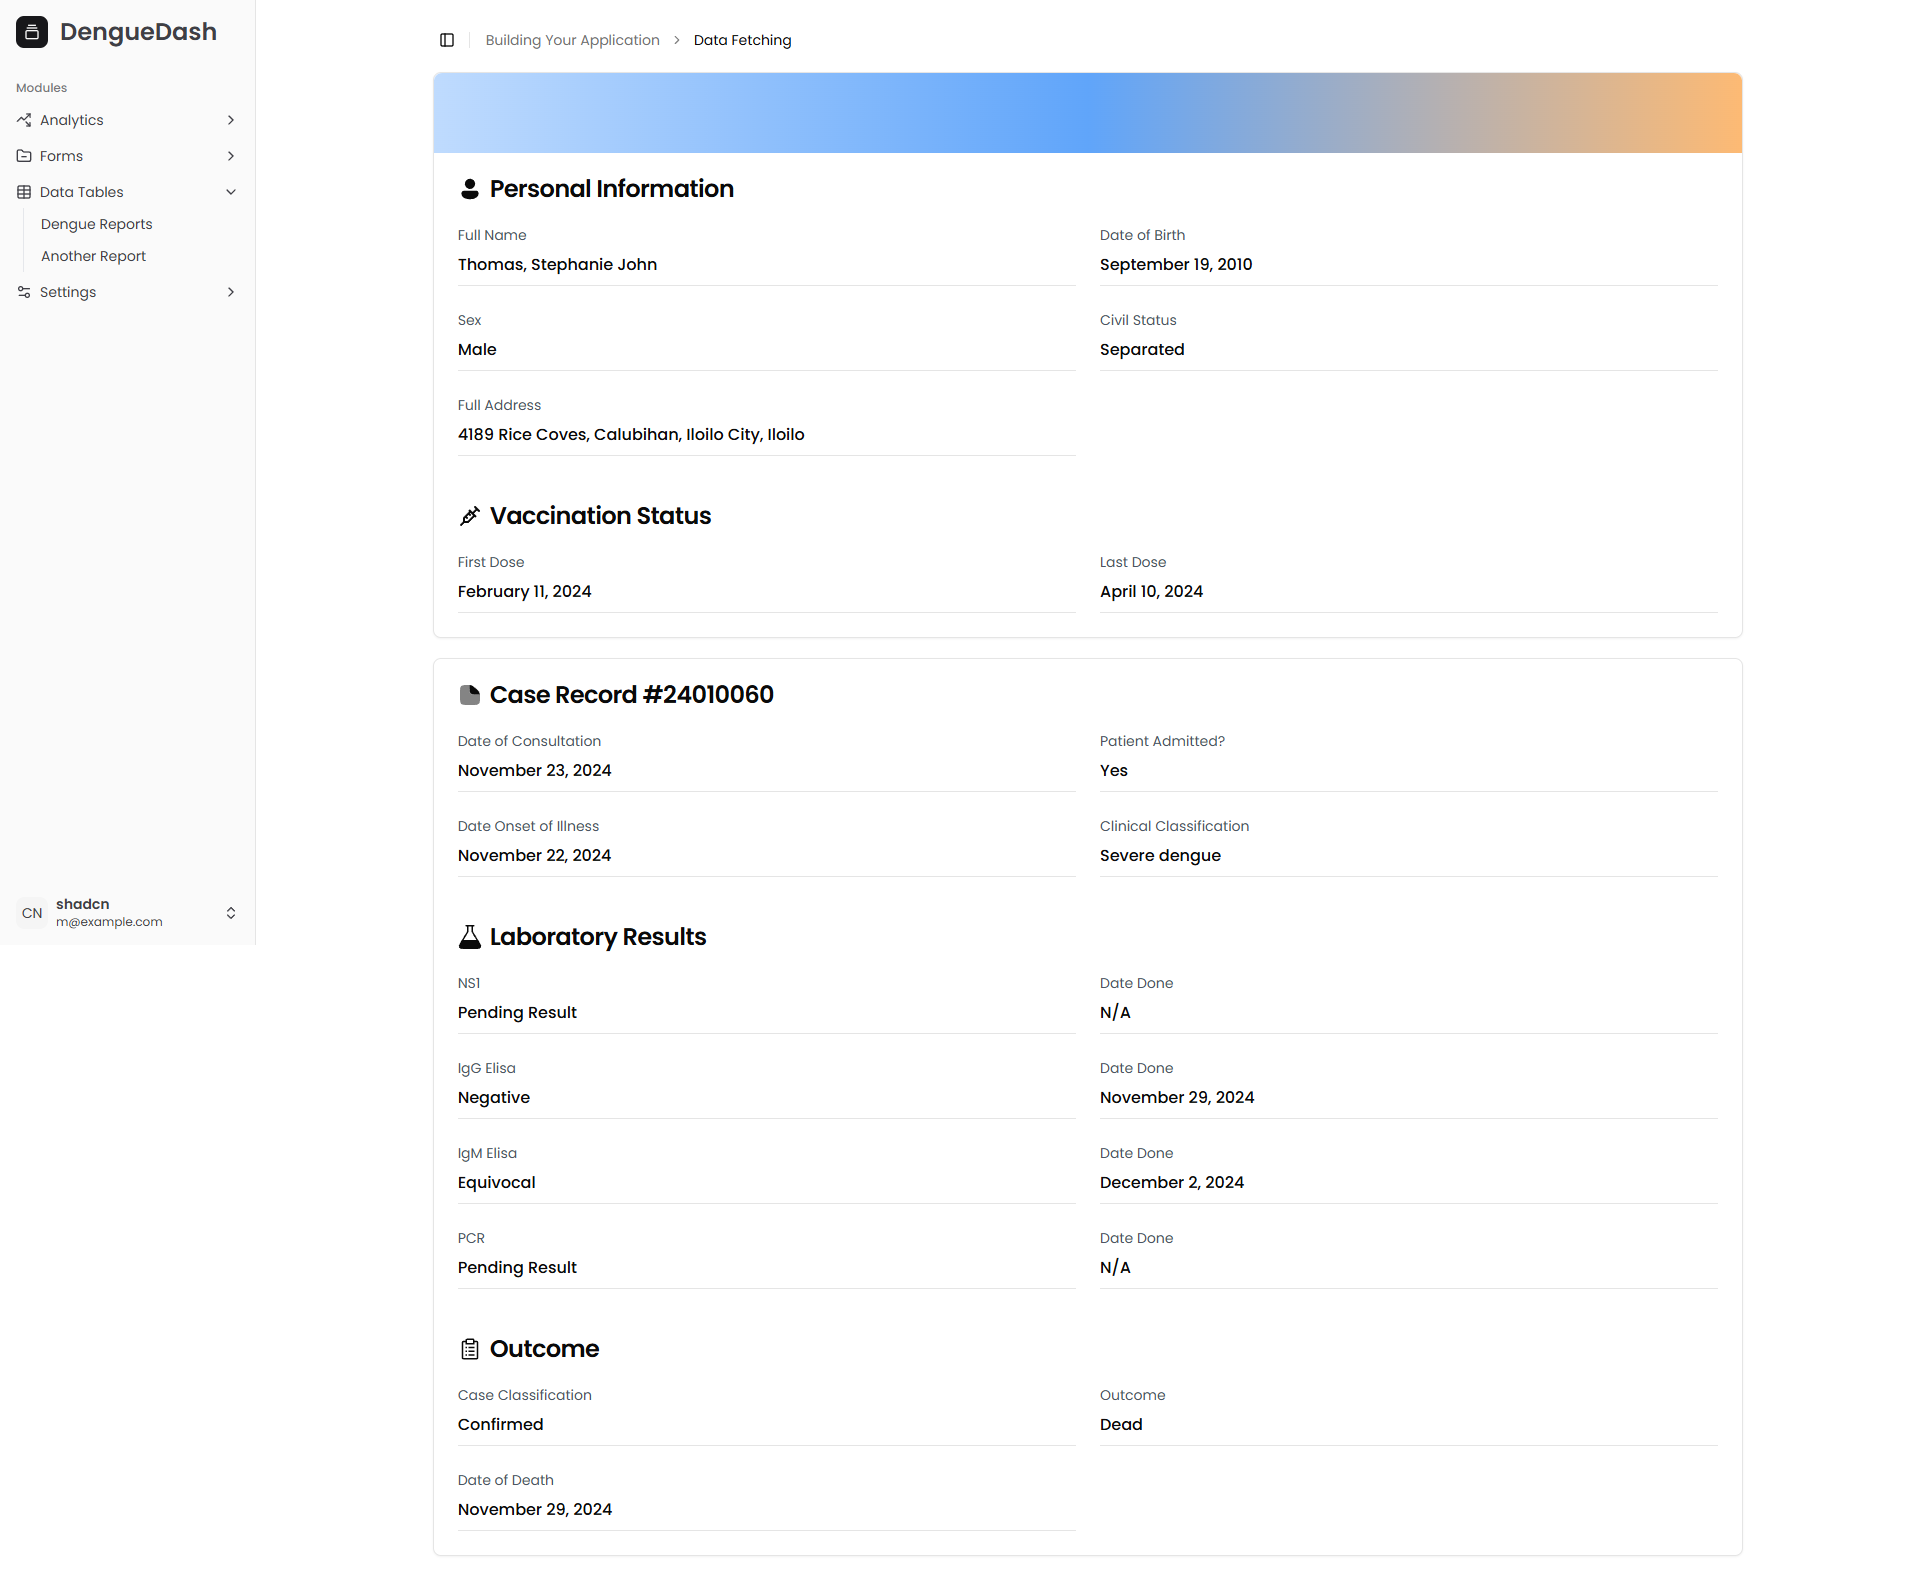
\includegraphics[width=1\textwidth]{case_report}
	\caption{Detailed Case Report}
	\label{fig:case_report}
\end{figure}
